\chapter{Background}
\label{ch:background}

This chapter provides the background knowledge relevant for the thesis work. It
will initially discuss graph and related problems (\autoref{sec:signed_graphs_and_density}) which are significant in the
following used methodologies, as well as concepts of computational complexity
(\autoref{sec:computational_complexity_and_approximability}) and Linear
Programming (\autoref{sec:linear_and_mixed_integer_programming}).

\section{Signed graphs and density}%
\label{sec:signed_graphs_and_density}

\section{Computational complexity and \\approximability}%
\label{sec:computational_complexity_and_approximability}

Complexity Theory deals with the study of the intrinsic complexity of
computational tasks; more specifically it mainly aims at determining the
complexity of any given task. It also elaborates on the relationships between
the complexity of different problems, for example proving that 2 problems are
computationally equivalent\cite{9780521884730}, through a notion called
\emph{reduction}.

\subsection{Complexity classes}%
\label{par:complexity_classes}

According to their complexity, problems can be divided in different groups
\cite{DemaineFall2014}.

\paragraph{$\mathcal{P} $}%
\label{par:p}
is the set of problems which can be solved in polynomial time in the size $n$ of
the problem, i.e. $n^{O(1)} $. In this set there are problems such as Linear
Programming Models \cite{KHACHIYAN198053}\cite{Karmarkar1984}, finding whether
or not a graph is connected \cite{9780521884730}.

\paragraph{$\mathcal{NP} $}%
\label{par:np} is the set of problems whose solution can be verified in
polynomial time in the size $n$ of the problem, i.e. $n^{O(1)} $.

According to these definition it is easy to see that $\mathcal{P} \subseteq
	\mathcal{NP} $. A common $\mathcal{NP} $ problem is factoring, i.e. finding a
prime factor $p$ of a number $N$ in a given interval \cite{SanjeevArora2017}.

\paragraph{$\mathcal{NP} $-Hard}%
\label{par:_np_hard} is the set of problems that are \emph{at least as hard} as
any other problem in $\mathcal{NP} $. Some well-known $\mathcal{NP} $-Hard
problems are the $\textsc{Sat}$ (deciding whether a boolean formula can be
satisfied or not) and the $\textsc{MaxClique}$ (finding the biggest complete
subgraph), as shown is a famous paper by Karp \cite{Miller1972} (see
\autoref{fig:tex/img/post_vaccine_social_scheduling} ).

\begin{figure}[]
	\centering
	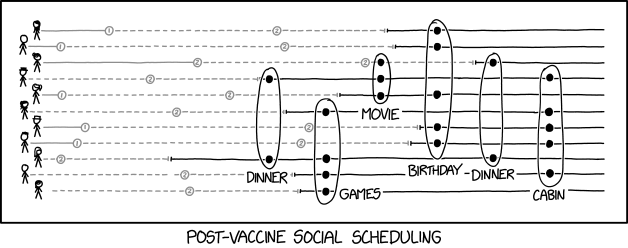
\includegraphics[width=0.8\linewidth]{tex/img/post_vaccine_social_scheduling.png}
	\caption{\emph{As if this problems weren't $\mathcal{NP} $-Hard enough}.
		Post-vaccine social scheduling may be $\mathcal{NP} $-Hard \cite{Munroe}}%
	\label{fig:tex/img/post_vaccine_social_scheduling}
\end{figure}

\paragraph{$\mathcal{NP} $-Complete}%
\label{par:_np_hard} is the set of problems in $\mathcal{NP} $-Hard that are
also in $\mathcal{NP} $. Intuitively these correspond the most difficult
problems to solve in $\mathcal{NP} $. The number of problems which are known to
be in this set is in the order of a thousand \cite{SanjeevArora2017}.

\subsection{$\mathcal{P} $ vs $\mathcal{NP}$}%
\label{sub:_p_vs_np_}

A fundamental question in Computational Complexity is wheter $\mathcal{P} =
	\mathcal{NP} $. Mostly people believe that this is not true, so
$\mathcal{P} \neq \mathcal{NP} $, and also our daily experience tell us that
often it is easier to check the correctness of a solution of a problem than
finding it \cite{9780521884730}: in many cases coming up with the correct
answer requires searching over an exponentially large set
\cite{SanjeevArora2017}. Nonetheless no mathematical proof of this notion has
been found and, in fact, in the last decades there has been little or no progress towards it \cite{Erickson2019}.

If, it is mostly accepted, $\mathcal{P} \neq \mathcal{NP} $ this would produce
a situation as depicted in \autoref{fig:tex/img/complexity-diagram}:
there are problems for which we are not able to find the solution
efficiently (i.e. in polynomial time). On the other side this allows the
existance of one-way-functions (i.e. functions whose inverse is much harder to
compute than the original functions) on which Modern Criptography heavily
relies \cite{9780521884730}.
%
% This brings the need for algorithms which are able to approximate the solution
% in a reasonable amount of time.

% Viceversa, if $\mathcal{P} = \mathcal{NP} $, it would be very easy to find
% proofs and mathematicians could be replaced by
% look at 2.7.3 in Sanjeev's book

\begin{figure}
	\centering
	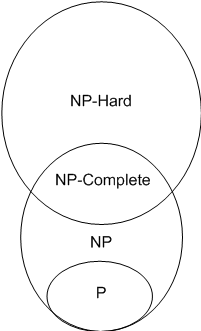
\includegraphics[width=0.3\linewidth]{tex/img/complexity-diagram.png}
	\caption{Venn diagram for the complexity classes if $\mathcal{P} \neq
			\mathcal{NP} $ \cite{article}}%
	\label{fig:tex/img/complexity-diagram}
\end{figure}

\subsection{Optimization Problems and $\mathcal{NPO} $}%
\label{sub:optimization_problems}

Optimization problems are defined from a problem instance $x$, a set of
feasible solutions $S$ and a cost function that takes as input the problem
instance $x$ a feasible solution $s \in S$, denoted as cost$_{O} (x, s) $.
Given a minimization (maximization) problem the optimal solution is defined as
the $s$ minimizing (maximizing) the value of cost$_{O} (x, s)$, and we denote
by opt$_{O} (x) $ this value\cite{Trevisan2004}.

\paragraph{$\mathcal{NPO} $}%
\label{par:_npo_}

is then the set of optimization problems whose cost function
can be computed in polynomial time and for every instance of the problem $x$
and feasible solution for that problem $s \in A$ there is a polynomial $q \; s.t.
	\; s \leq q(|x|)$ (i.e. the size of every solution is bounded by a polynomial
in $x$).

If $\mathcal{P} \neq \mathcal{NP} $ for many optimization problems there is no
algorithm for finding the optimal solution in polynomial time
\cite{Trevisan2004}. This is again a fundamental limitation about what we can
compute which then requires the definition of some alternative approaches, like
the definition of \emph{approximation algorithm}
which are able to be computed in polynomial time
a solution which lies in a given factor from the optimal
one\cite{Vazirani2002}.

\paragraph{Approximation}%
\label{par:r_approximations}

$A$ is an r-approximation algorithm for an $\mathcal{NPO} $ minimization
problem $O$ if, for every instance $x$ of $O$ it holds that
\begin{equation*}
	cost_{O} (x, (A(x))) \leq r \cdot opt_{O} (x)
\end{equation*}

\noindent
(or, respectively, cost$_{O} (x, (A(x)))
	\leq 1/r \cdot $opt$_{O} (x) $ for maximization problems), $A(x)$ being the
optimal solution found by the approximation algorithm \cite{Trevisan2004}.

\subsection{Approximation preserving reductions}%
\label{sub:approximation_preserving_reductions}

Problems approximability varies widely: while for some of them exists
constant factor approximations, for some others even a remotely approximate
solution cannot be found \cite{Ausiello2005} (some examples are listed in
\autoref{tab:inapproximability-examples} ).

% todo: reference to the papers proving each result instead of the hub
\begin{table}
	\centering
	\caption{Examples of known inapproximability results, assuming $\mathcal{P}
			\neq \mathcal{NP} $ \cite{10.1007/3-540-63248-4_10} }
	\label{tab:inapproximability-examples}
	\begin{tabular}{c|p{5cm}|c}
		Problem                                                          & Description                                                   & Inapproximability \\
		\hline
		$ \textsc{MaxClique} $                                           & Biggest complete subgraph                                     & $|V|^{1-
		\epsilon}, \forall \epsilon > 0 $                                                                                                                    \\
		                                                                 &                                                               &                   \\
		$ \textsc{MaximumIndipendentSet} $                               &
		Biggest set of not connected nodes                               & $|V|^{1-
		\epsilon}, \forall \epsilon > 0 $                                                                                                                    \\
		                                                                 &                                                               &                   \\
		$ \textsc{MinCut} $                                              & Partition of nodes in 2 sets $V_1$ and $V_2$ minimizing edges
		between the 2 sets                                               & 1.0624                                                                            \\
		                                                                 &                                                               &                   \\
		$ \textsc{MaximumSetPacking} $                                   & Given a collection of
		finite sets $C$,
		finding the biggest collection $C' \subseteq C$ of disjoint sets & $|C|^{1-
		\epsilon}, \forall \epsilon > 0 $                                                                                                                    \\
	\end{tabular}
\end{table}

\emph{Approximation preserving reductions} are a fundamental notion for proving
a partial order among optimization problems \cite{Ausiello2005}. An
\emph{Approximation preserving reductions} must have
the following properties (when reducing from a problem $A$ to a problem $B$)
\cite{DemaineFall2014}:

\begin{itemize}
	\item any instance $x$ of $A$ should be mapped to an instance $x' = f(x)$
	      of $B$ in polynomial time
	\item any solution $y'$ of $B$ should be associated to a corresponding
	      solution $y = g(y')$ of $A$ in polynomial time
\end{itemize}

So there are 2 feasible (i.e. requiring polynomial time) functions $f$ and $g$
for mapping instances of $A$ to $B$ and solution of $B$ to solutions of $A$,
respectively.

There are different kinds of approximation preserving reductions.

\subsubsection{Strict reductions}%
\label{sub:strict_reductions}

% \subsubsection{L reductions}%
% \label{sub:l_reductions}

\section{Linear and Mixed Integer Programming}%
\label{sec:linear_and_mixed_integer_programming}
